\section{Experiment}\label{sec:Experiments}

We deploy an HDFS cluster to evaluate EarnCache's performance, on which Spark and EarnCache are deployed as the upper-level application tier and the middle-level caching tier respectively.
The cluster consists of five Amazon EC2 m4.2xlarge nodes, one of which \textcolor{red}{serves} as the masters of Spark, EarnCache and the underlying HDFS, four of which serves as slaves of Spark, EarnCache and HDFS.
Each cluster node has 32GB \textcolor{red}{of} memory, \textcolor{red}{12GB reserved as working memory and the remaining 20GB of memory employed as cache resources, summing up to 80GB of cache in total.}
%and 12GB memory is reserved as working memory, and the remaining 20GB memory is employed as cache resources, meaning that EarnCache's cache capacity is 80GB.

We mainly evaluated EarnCache's performance by issuing jobs from Spark to scan cached files parallelly \textcolor{red}{\sout{while}} without any further processing, and compare the performance of EarnCache incremental caching with LRU, LFU on-demand caching and with the MAX-MIN fair caching. We set the observation window size of EarnCache to 1000GB by default. For each experiment, we issue file scanning jobs on three cached files, denoted as FILE-1, FILE-2 and FILE-3, with the following three various frequency patterns, denoted as ROUND, ONE and TWO respectively.
\begin{itemize}
\item ROUND Three files are accessed in pattern: FILE-1, FILE-2,FILE-3 ..., where three files are accessed with equal frequency.
\item ONE Three files are accessed in pattern: FILE-1, FILE-2, FILE-1, FILE-3 ..., where one file is accessed more frequently than other two files.
\item TWO Three files are accessed in pattern: FILE-1, FILE-2, FILE-1, FILE-2, FILE-3 ..., where two files are accessed more frequently than the other file.
\end{itemize}

We respectively set the size of FILE-1, FILE-2 and FILE-3 equally to 40GB and unequally to 70GB, 40GB and 10GB, and then evaluate EarnCache with different caching strategies and different frequency patterns. Fig.~\ref{fig:2-a} and Fig.~\ref{fig:2-b} shows the averaged overall running time of jobs scanning various number of \textcolor{red}{equally and unequally sized} files within one period of ROUND, ONE and TWO frequency patterns, \textcolor{red}{including $3$, $4$, and $5$ file scans each}. We can see that EarnCache provides the best file scanning performance,

\begin{figure}[!htbp]
    \subfigure[Files with equal size]{
    		\begin{minipage}[b]{0.47\linewidth}
    		\centering
    		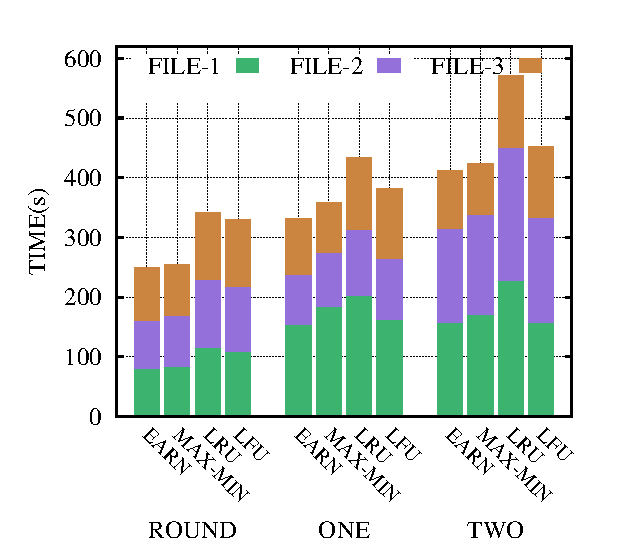
\includegraphics[scale=0.41]{figures/scan444_time_all.eps}
            \label{fig:2-a}
    		\end{minipage}
    }
    \subfigure[Files with unequal size]{
        \begin{minipage}[b]{0.47\linewidth}
        \centering
        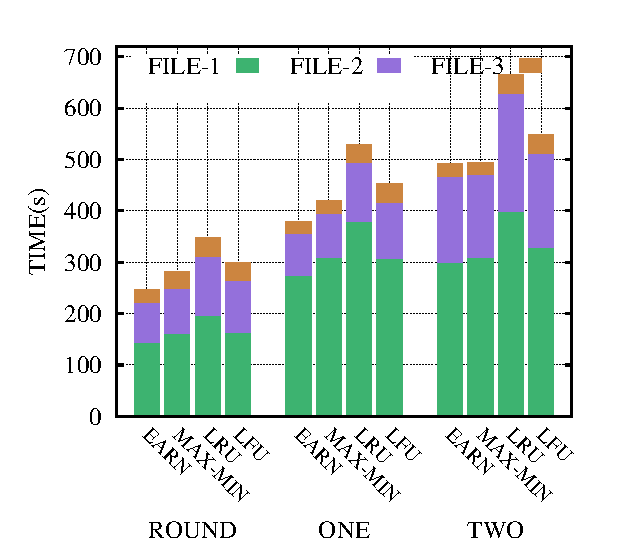
\includegraphics[scale=0.41]{figures/scan741_time_all.eps}
        \label{fig:2-b}
        \end{minipage}
    }
    \caption{Running time of file scanning jobs.}
    \label{fig:2}
\end{figure}

More specifically, we statistically analyze the distribution of blocks accessed from local cache, from remote cache, and from the under distributed file system respectively, and the results are shown in Fig.~\ref{fig:block_count}. We can see that EarnCache has the largest number of blocks accessed from cache, locally or remotely, which means that it yields the highest memory efficiency than other caching strategies, and this self-evidently explains why EarnCache yields the best file scanning performance. However, we can see that EarnCache is the strategy which has the largest number of blocks accessed from remote cache among the four evaluated strategies. The reason is that \textcolor{red}{the Spark task scheduler is not optimized to recognize blocks in exclude cache and under file system in seperate.}
and this also means EarnCache has the largest potential of performance improvement. If cache-aware task scheduling can be injected into the upper-level task scheduler, more tasks could access their input data blocks from local cache, and EarnCache could obtain much better overall performance than other caching strategies.

\begin{figure}[!htbp]
    \centering
    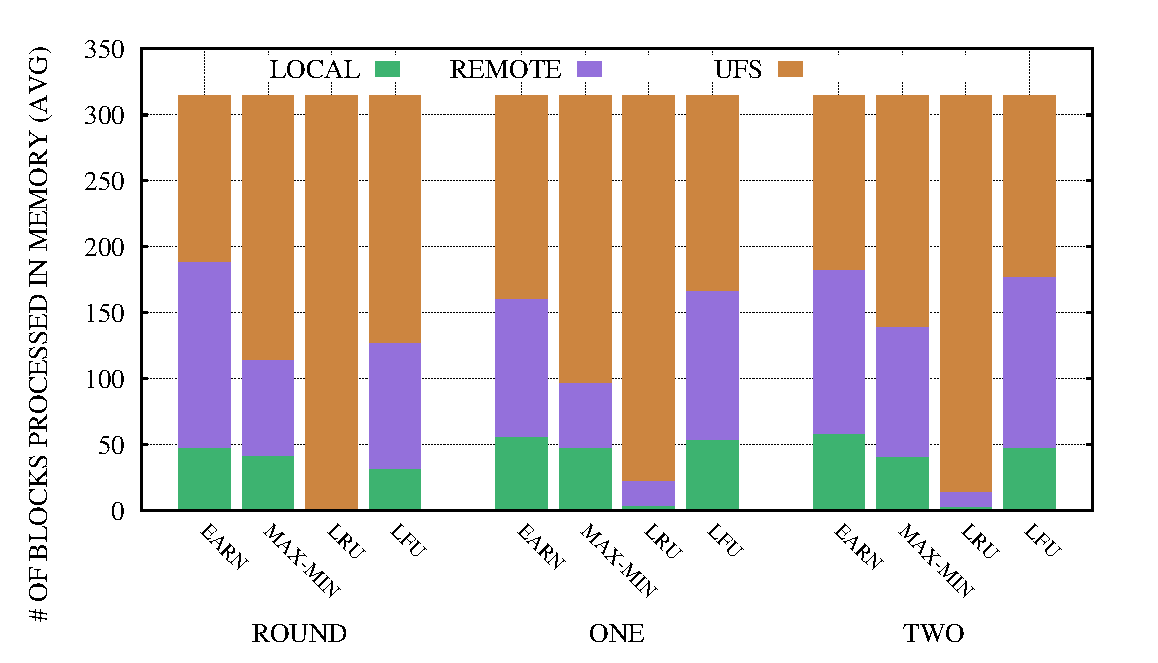
\includegraphics[scale=0.43]{figures/block_count_avg.eps}
    \caption{Distribution of blocks accessed in local cache, remote cache and under file system.}
    \label{fig:block_count}
\end{figure}

We can also see that the performance of EarnCache is only slightly better than the MAX-MIN caching strategy, and sometimes they achieve similar performance. This is because that file receives moderately divergent amounts of cache resources with these two caching strategies, as far as our experimental settings are concerned. However, the MAX-MIN caching is unable to re-allocate resources properly when there exist files not receiving any further accesses. To illustrate this, we comparatively present the process of resource re-allocation of EarnCache and the MAX-MIN caching in Fig.~\ref{fig:3-2-a} and Fig.~\ref{fig:3-2-b}, when two out of three equal-sized files stop receiving further accesses. We can see that the file remaining accessed gradually takes over cache resources from those obsolete files as time goes on, while each file with MAX-MIN caching still equally holds 1/3 cache resources even though two files receives no further accesses. Correspondingly, the running time of the file scanning job gradually decreases with EarnCache, while remains stable with MAX-MIN caching.  

%\begin{figure}[!htbp]
%    \subfigure[EARN]{
%    		\begin{minipage}[b]{0.47\linewidth}
%    		\centering
%    		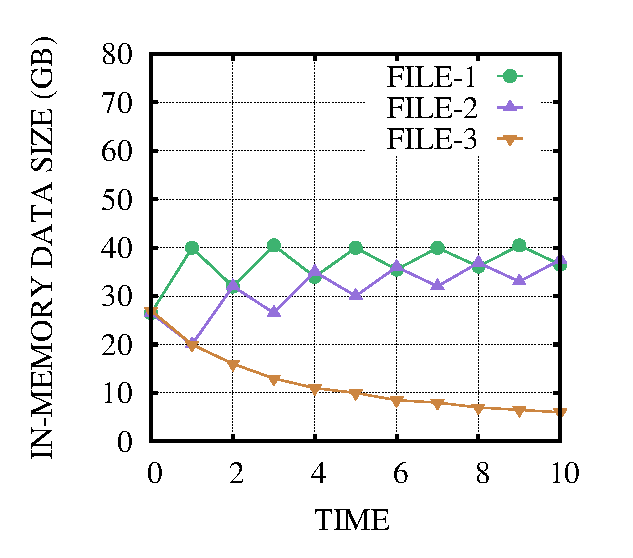
\includegraphics[scale=0.41]{figures/3-1-earn-1000-ds.eps}
%    		\end{minipage}
%    }
%    \subfigure[MAX-MIN]{
%        \begin{minipage}[b]{0.47\linewidth}
%        \centering
%        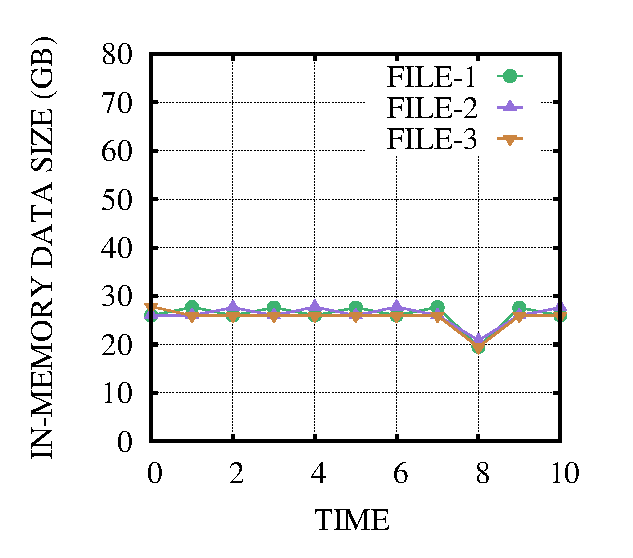
\includegraphics[scale=0.41]{figures/3-1-maxmin-1000-ds.eps}
%        \end{minipage}
%    }
%    \caption{Cache resource In-memory data size of each file after File-3 stops been visited.}
%    \label{fig:3-1}
%\end{figure}


\begin{figure}[!htbp]
    \subfigure[EARNCache]{
    		\begin{minipage}[b]{0.47\linewidth}
    		\centering
    		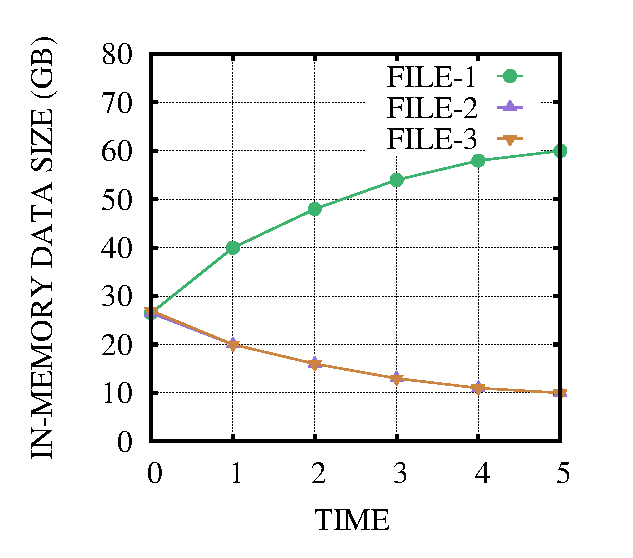
\includegraphics[scale=0.41]{figures/3-2-earn-1000-ds.eps}
            \label{fig:3-2-a}
    		\end{minipage}
    }
    \subfigure[MAX-MIN]{
        \begin{minipage}[b]{0.47\linewidth}
        \centering
        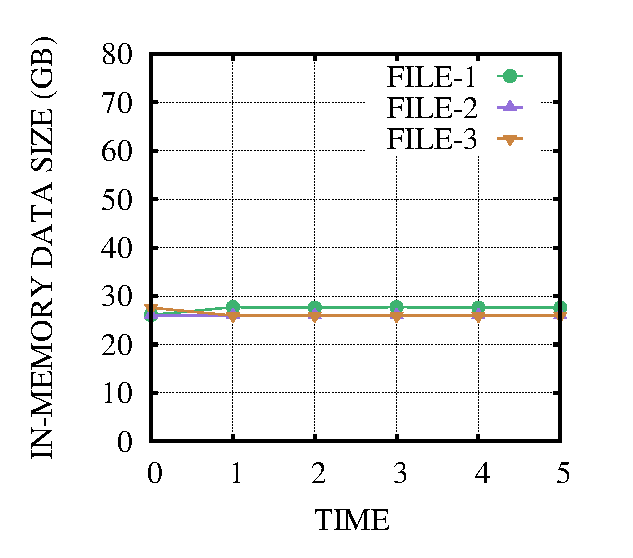
\includegraphics[scale=0.41]{figures/3-2-maxmin-1000-ds.eps}
        \label{fig:3-2-b}
        \end{minipage}
    }
    \caption{Dynamic resource re-allocation with two files receiving no further accesses.}
    \label{fig:3-2}
\end{figure}

Finally, we experimentally analyze the impact of the predefined observation window size on the average running time of file scanning jobs, and the results are presented in Fig.~\ref{fig:time_windowsize}.  We can see that when the observation window size is set too small, the time performance will degrade.

\begin{figure}[!htbp]
\centering
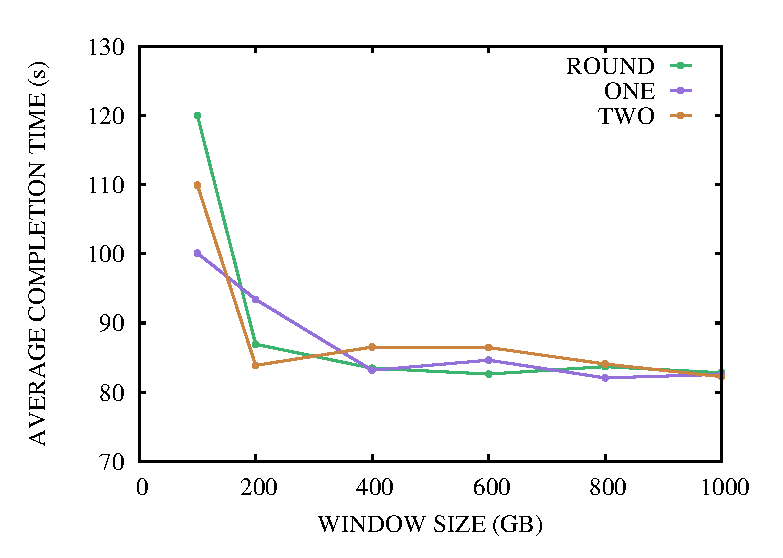
\includegraphics[scale=0.41]{figures/window_size_time.eps}
\caption{Impact of the observation window size.}
\label{fig:time_windowsize}
\end{figure} 